\section{Introduction}
The study of relativistic heavy-ion collisions provides a fruitful playground for physicists to understand many different aspects of high-energy nuclear physics ranging from the resolution of the complex nuclear structure to the highly interesting physics of the Quark-Gluon-Plasma (QGP) providing further insights into to state of the art of our Universe shortly after the Big Bang. \\
A complete treatment of these collision events would need concepts from quantum chromodynamics (QCD), relativistic hydrodynamics and also methods from statistical physics. Here we will focus on the latter since the aim of this seminar is to get insights into the various applications of the concepts presented in the introductory lecture on statistical physics and the previous talks to modern research.\\
For a visualization of the complexity of the physical processes relevant for the study of relativistic heavy-ion collisions have a look at figure \ref{fig:phases} at the beginning of the next page. In this talk we will have a closer look at the initial stages of such events since only a detailed understanding of the relaxation of the out-of-equilibrium initial state into a (hopefully) known equilibrium final state allows further analysis using the well-known techniques from e.\,g. hydrodynamics mentioned before (and displayed in the upper part of the corresponding figure). \newpage
\begin{figure}[t]
\centering
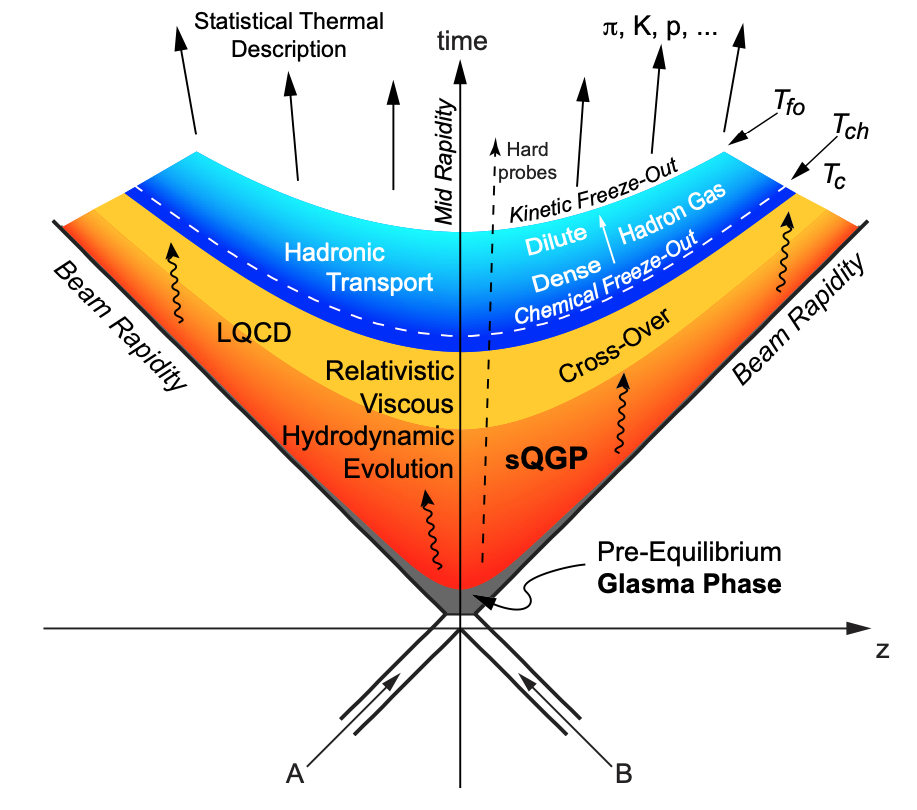
\includegraphics[width = 0.5\textwidth]{figures/rhic_schematic}
\caption[Visualization of the spacetime evolution of the system created in relativistic heavy-ion collisions.]{Visualization of the spacetime evolution of the system created in relativistic heavy-ion collisions. We will focus on the pre-equilibrium phase which is displayed here in the gray area near the origin.\footnotemark }
\label{fig:phases}
\end{figure}
\footnotetext{The figure was taken from B. Hippolyte's slides: \tiny{\url{http://www.nupecc.org/presentations/hippo_mar17.pdf} (23.06.2020)}}
